
\subsection{Vectorcardiogram dataset}  \label{sec:vcg_np}

The vectorcardiogram is a loop traced by the {cardiac vector} during a cycle of the heart beat. The two directions of orientation of this
loop in three dimensions form a point on the Stiefel manifold. The dataset of~\cite{vecdata} includes $98$ such recordings,
and is displayed in the left panel of Figure \ref{fig:vcg_data}. We represent each observation with a pair of orthonormal vectors, with the cone of 
lines to the right forming
the first component. This empirical distribution 
possesses a single mode, so that
the matrix Langevin distribution seems a suitable model.
  \begin{figure}
  \centering
  \begin{minipage}{0.5\textwidth}
    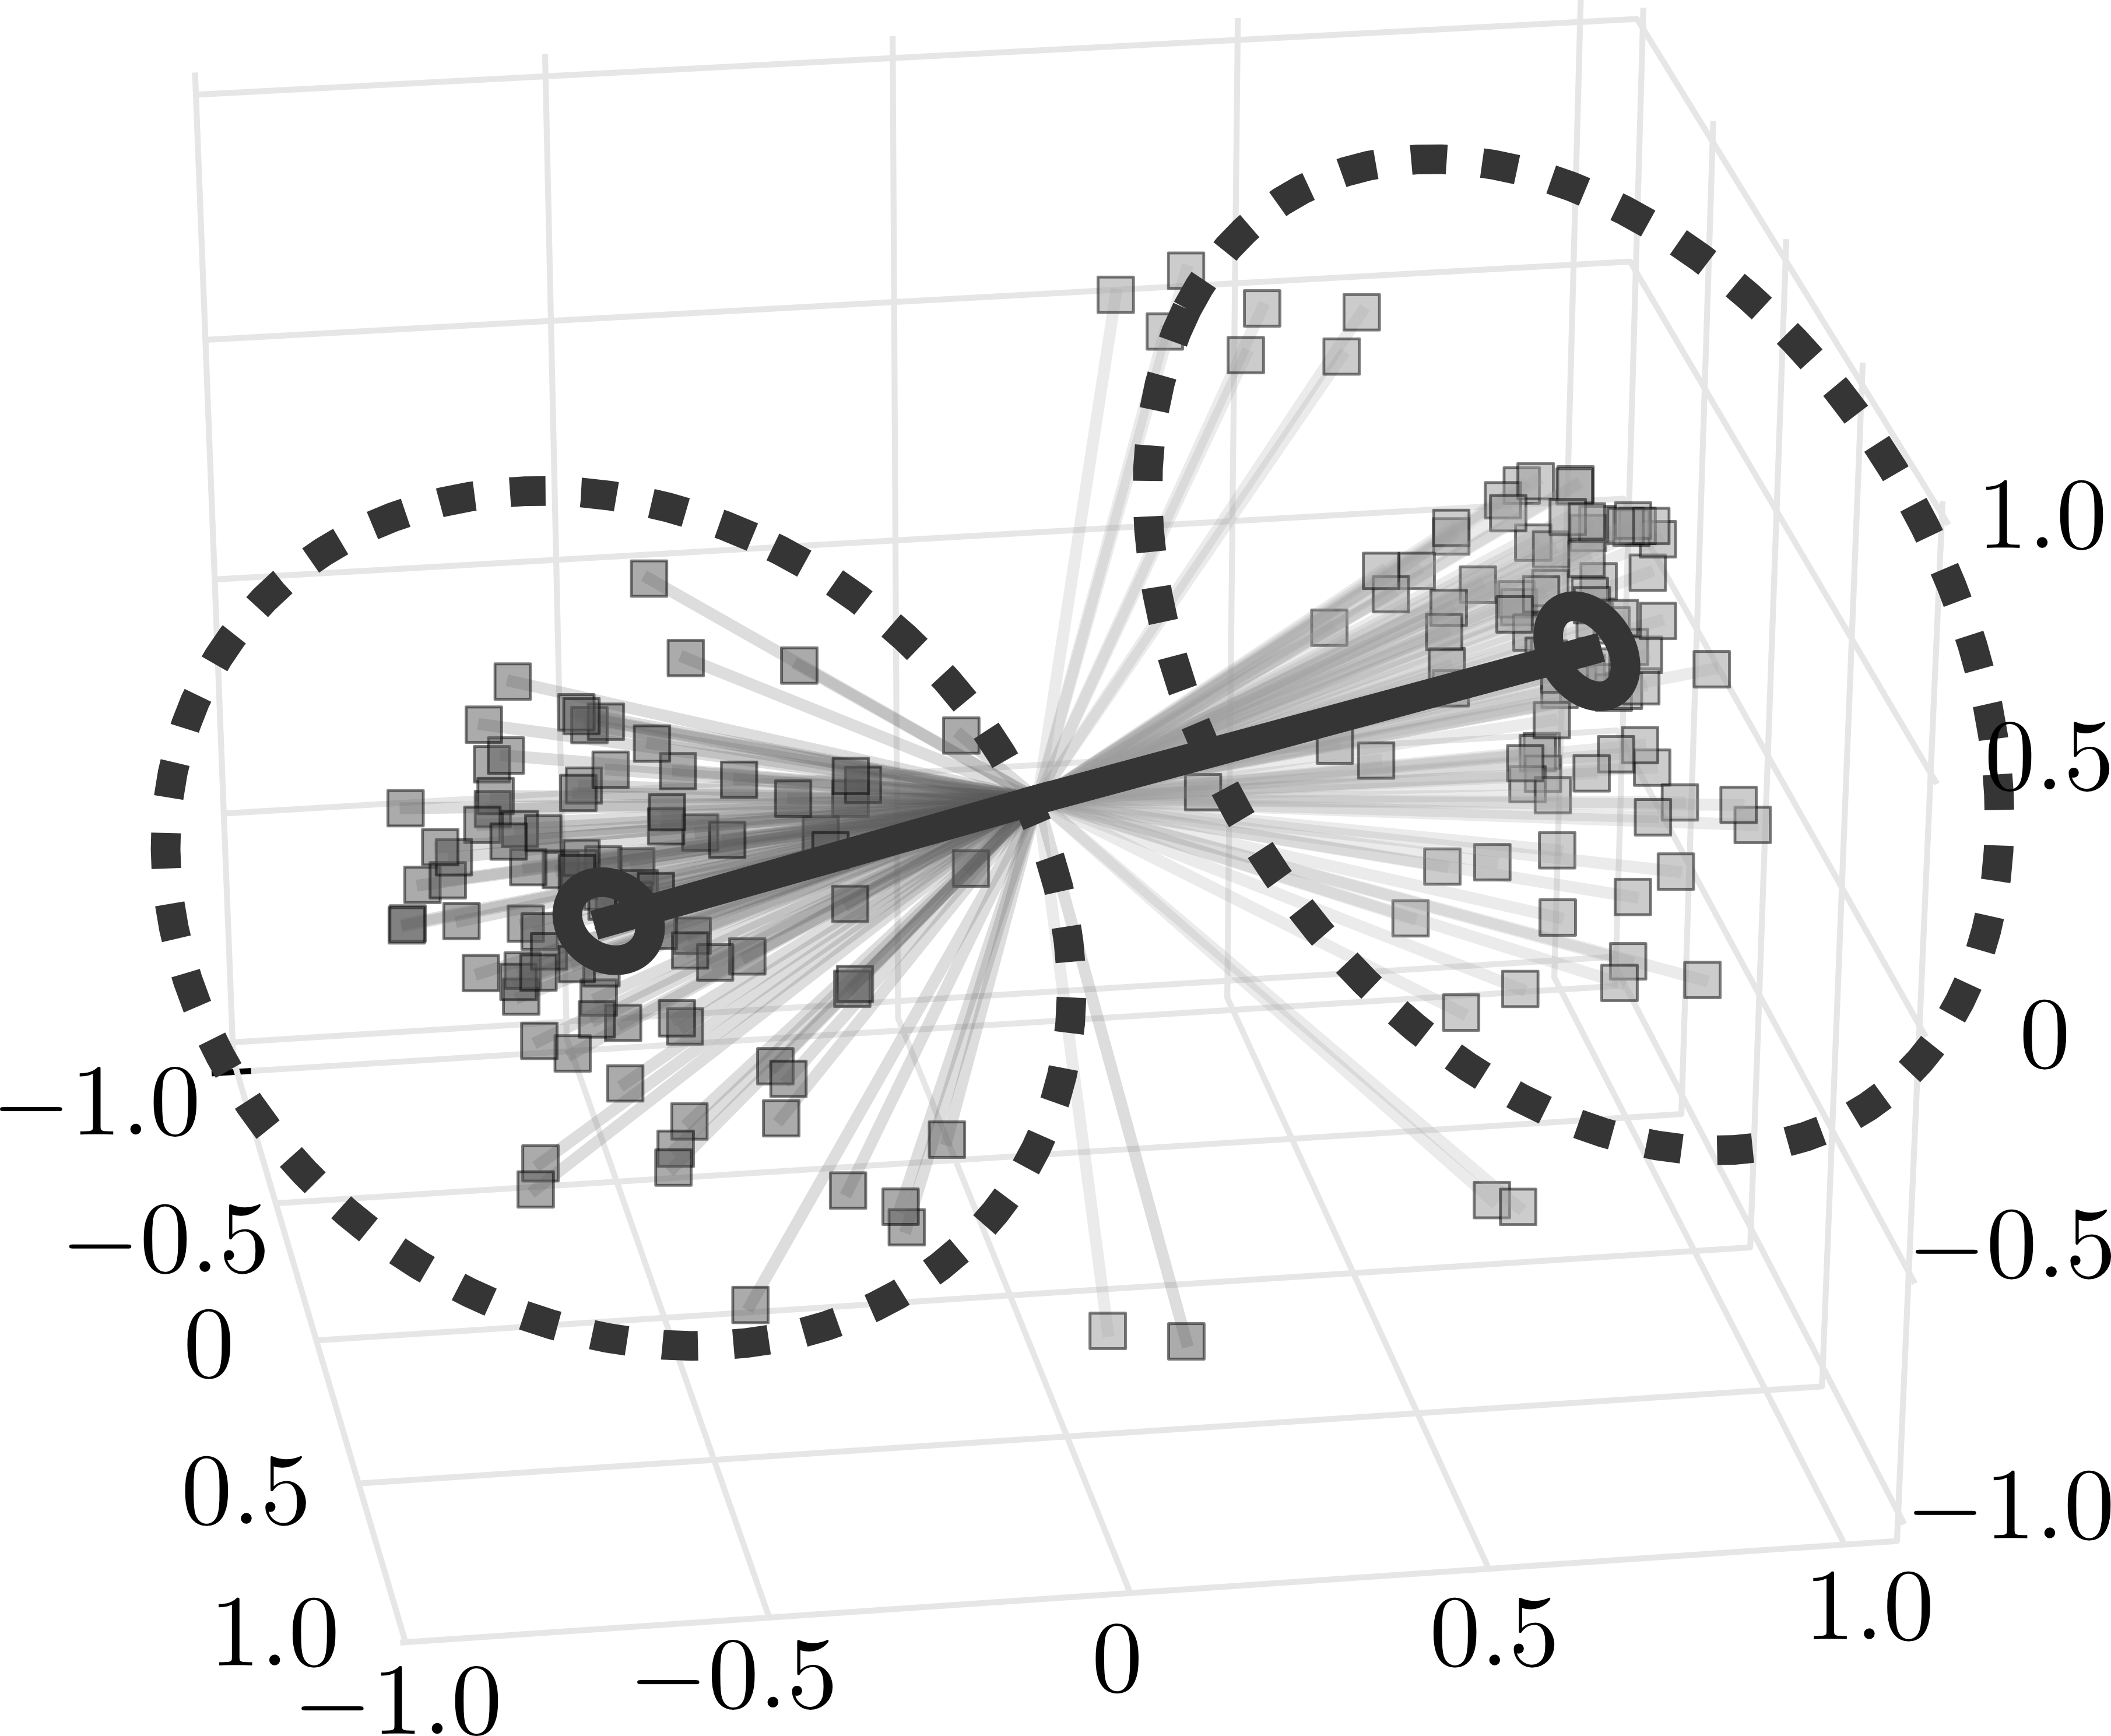
\includegraphics{figs/plot_vcg_post_bw2.png}
  \end{minipage}
  \begin{minipage}{0.4\textwidth}
  \centering
    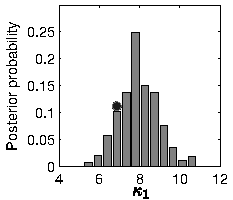
\includegraphics{figs/plot_vcg_kap1_bw.pdf}
  \centering
    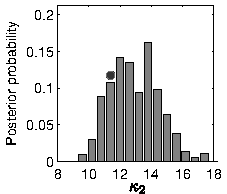
\includegraphics{figs/plot_vcg_kap2_bw.pdf}
  \end{minipage}
\caption{(Left) Vector cardiogram dataset with inferences. Bold solid lines are maximum likelihood estimates of $G$, and solid circles
 contain $90\%$ posterior mass. Dashed circles are $90\%$ predictive probability regions.
 (Right) Posterior distribution over $\kappa_1$ and $\kappa_2$, circles are maximum likelihood estimates.}
  \label{fig:vcg_data}
  \end{figure}

We place independent exponential priors with mean 10 and variance 100 on the scale parameter $\bkappa$, and a uniform prior on the location
parameter $G$. We restrict $H$ to be the identity matrix. Inferences were carried out using the Hamiltonian sampler to produce 10,000 samples, with a
burn-in period of 1,000. For the leapfrog dynamics, we set a step size of $0.3$, with the number of steps equal to 5.
We fix the mass parameter to the identity matrix.
We implemented all algorithms in $\mathtt{R}$, building on
the $\mathtt{rstiefel}$ package of~\cite{hoff2009}. 
Simulations were run on an Intel Core 2 Duo 3 Ghz CPU.
%The right plot in Figure \ref{fig:vcg_param1} shows the posterior distribution over the first component of $\bkappa$, which is centered around $1.75$
%(the second component is similar).
For comparison, we include the maximum likelihood estimates of $\bkappa$ and $G$. %; see the appendix for more details on this.
For  $\kappa_1$ and $\kappa_2$, these were $11.9$ and $5.9$, and we plot these in the right half of Figure \ref{fig:vcg_data}
as circles. 

%The blue bars show the
%Bayesian posteriors over the components of $G$.
The bold straight lines in Figure \ref{fig:vcg_data}, left, show the maximum likelihood estimates of the components of $G$, with the small
circles corresponding to $90\%$ Bayesian credible regions
estimated from the Monte Carlo output.
The dashed circles correspond to $90\%$ predictive probability regions for the Bayesian model. For these, we generated  $50$ points on $V_{3,2}$ for 
each sample, with parameters specified by that sample. The dashed circles contain $90\%$ of these points across all samples.
Figure \ref{fig:vcg_data}, right, shows the posterior over $\kappa_1$ and $\kappa_2$.

\subsection{Comparison of exact samplers} \label{sec:Bayes_expt}

%Here, we compare our sampler with the exchange sampler
%for the matrix Langevin distribution.
%the exchange sampler and our sampler based on the rejection sampler underlying the Matrix Langevin distribution.
To quantify sampler efficiency, % we explore parameter space, 
we estimate the
effective sample sizes produced per unit time. This corrects for
correlation between successive Markov chain samples
by estimating the number of independent samples produced; for this
we used the $\mathtt{rcoda}$ package of~\cite{Rcoda2006}.
%We evaluate these on the vectorcardiogram dataset.

  \begin{figure}
  \centering
    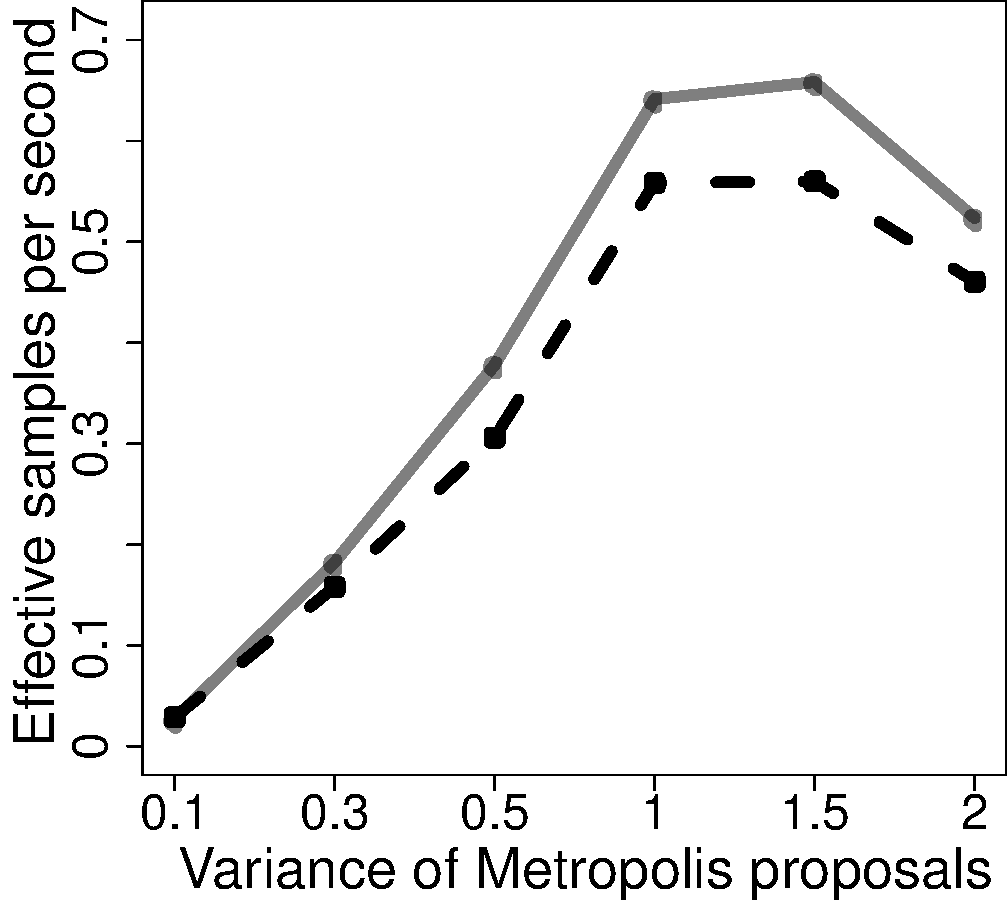
\includegraphics[width=.3\textwidth]{figs/mh_plot_bw.pdf}
  \centering
    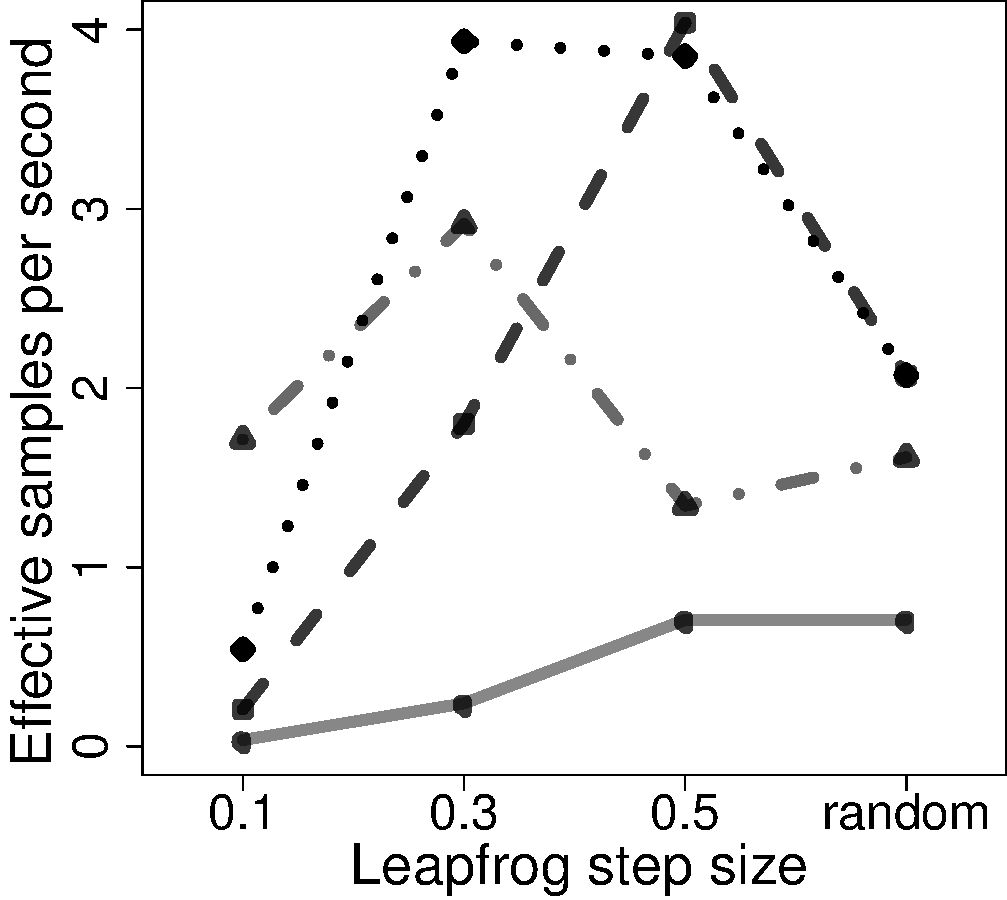
\includegraphics[width=.3\textwidth]{figs/hmc_plot_bw.pdf}
\caption{Effective samples per second for (left) random walk and (right) Hamiltonian samplers. From bottom to top at abscissa $0.5$: (left) 
 Metropolis--Hastings data-augmentation sampler and exchange sampler, and 
 (right) 1, 10, 5 and 3 leapfrog steps of the Hamiltonian sampler.}
  \label{fig:samplers_comp}
  \end{figure}

The left panel in Figure \ref{fig:samplers_comp} shows the effective sample size per second for two
Metropolis--Hastings samplers, the exchange sampler and our latent variable sampler on the vectorcardiogram dataset.
% based on
%the rejection sampler of \cite{hoff2009}. % underlying the Matrix Langevin distribution.
Both 
perform a random walk in the $\bkappa$-space, with the steps drawn for a normal
distribution whose variance increases along the horizontal axis.
%The vertical axis shows the
%median effective sample size per second for the components of $\bkappa$.
The figure shows that both samplers' performance
peaks when the proposals have a variance between $1$ and $1.5$, with the
exchange sampler performing slightly better. However, 
the real advantage of our sampler is that introducing the latent variables
results in a joint distribution with no intractable terms,
allowing the use of more sophisticated sampling algorithms. The right panel studies the Hamiltonian
Monte Carlo sampler described at the end of Section \ref{sec:latent_hist}. Here we
vary the size of the leapfrog steps along the horizontal axis, with the different
curves corresponding to different numbers of such steps.
This performs an order of magnitude better than either of the previous
algorithms, with performance peaking with $3$ to $5$ steps of size $0.3$ to
$0.5$, fairly typical values for this algorithm. This shows the advantage of exploiting
gradient information in exploring the parameter space.


\subsection{Comparison with an approximate sampler}
In this section, we consider an approximate sampler based on an asymptotic approximation to 
$Z(\bkappa)= \mathstrut_0F_1(d/2, \bkappa^T\bkappa/4)$ for large values of
$(\kappa_1, \ldots, \kappa_n)$~\citep{khatri1977}:
\begin{align}
  Z(\bkappa)  \simeq &
         \left\{ \frac{2^{-\frac{1}{4}p(p+5) + \frac{1}{2}pd}}{\pi^{\frac{1}{2}p}} \right\} \etr(\bkappa) \prod_{j=1}^p \Gamma\left(\frac{d-j+1}{2} \right)
   \left[ \left\{\prod_{j=2}^p \prod_{i=1}^{j-1}(\kappa_i + \kappa_j)^{\frac{1}{2}} \right\} \prod_{i=1}^p \kappa_i^{\frac{1}{2}(d-p)} \right]^{-1}. \nonumber
\end{align}
%An expansion, similar in spirit, but for the matrix Bingham distribution was used by \cite{hoff2009jrssb}. 
We use this approximation in the acceptance probability
of a Metropolis--Hastings algorithm; it can similarly be used to construct a Hamiltonian sampler. 
For a more complicated but accurate approximation, see~\cite{Kume:2013:SAN}. In general however, using
such approximate schemes involves the ratio of two approximations, and can
have very unpredictable performance. %Below, we study the behaviour of this approximation along with the performance of our exact sampler.
  \begin{figure}
  \centering
    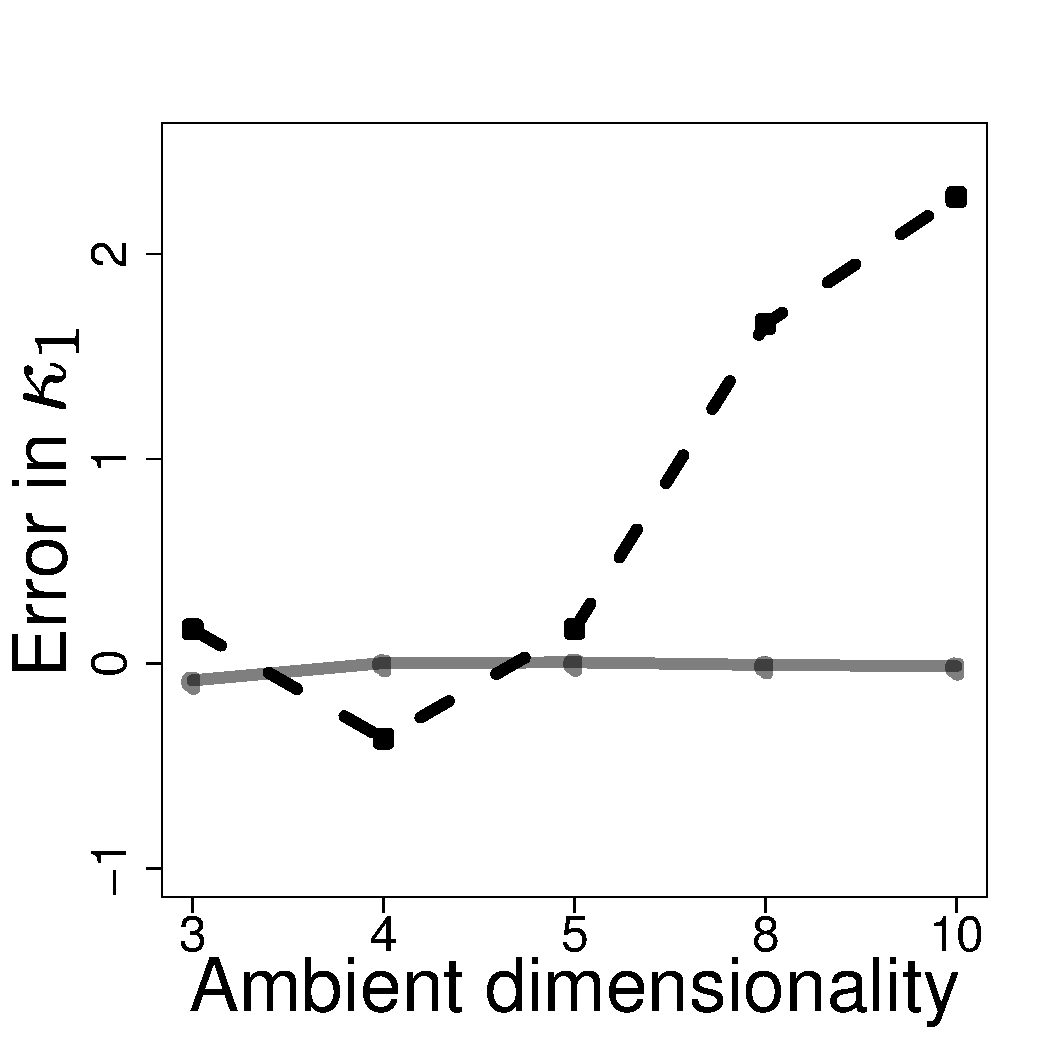
\includegraphics[width=.25\textwidth]{figs/approx_err1_bw.pdf}
  \centering
    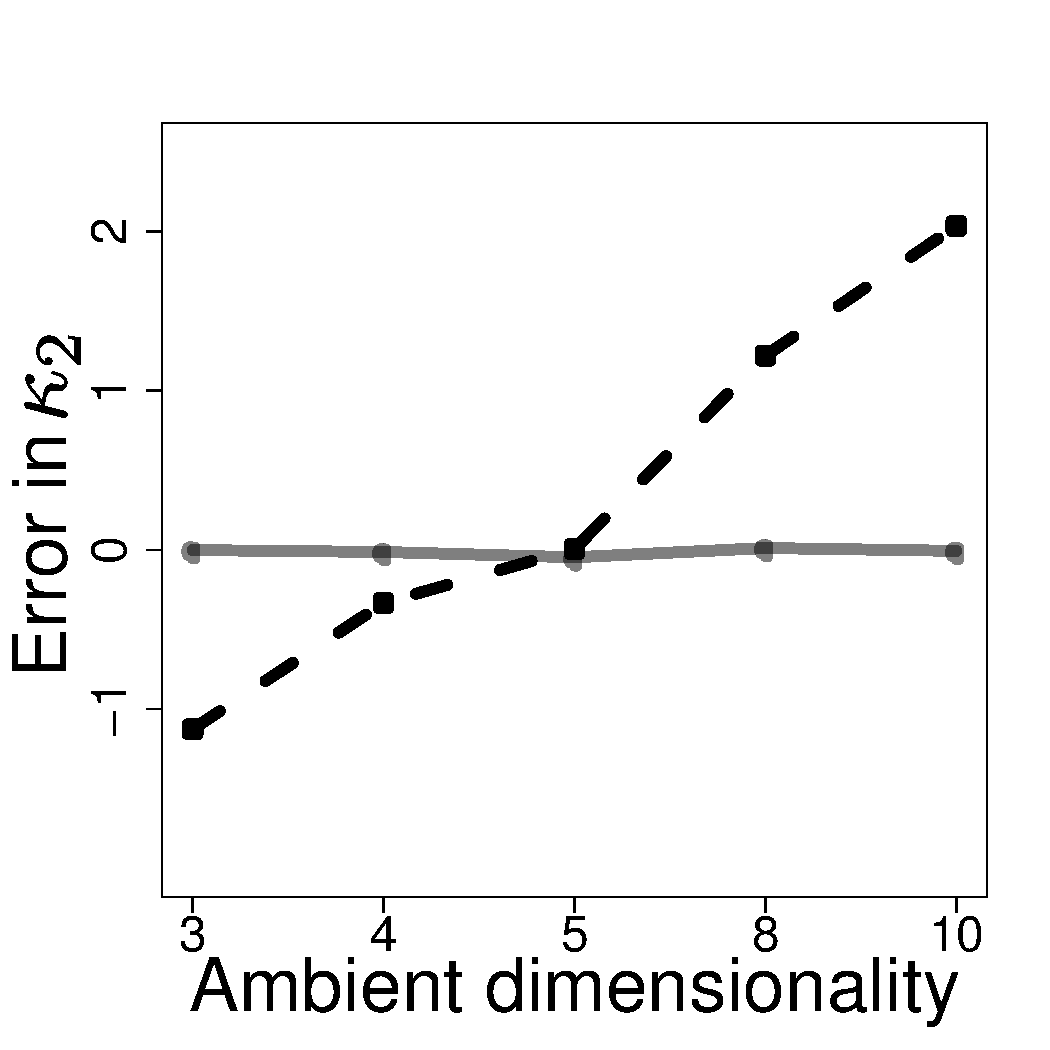
\includegraphics[width=.25\textwidth]{figs/approx_err2_bw.pdf}
  \centering
    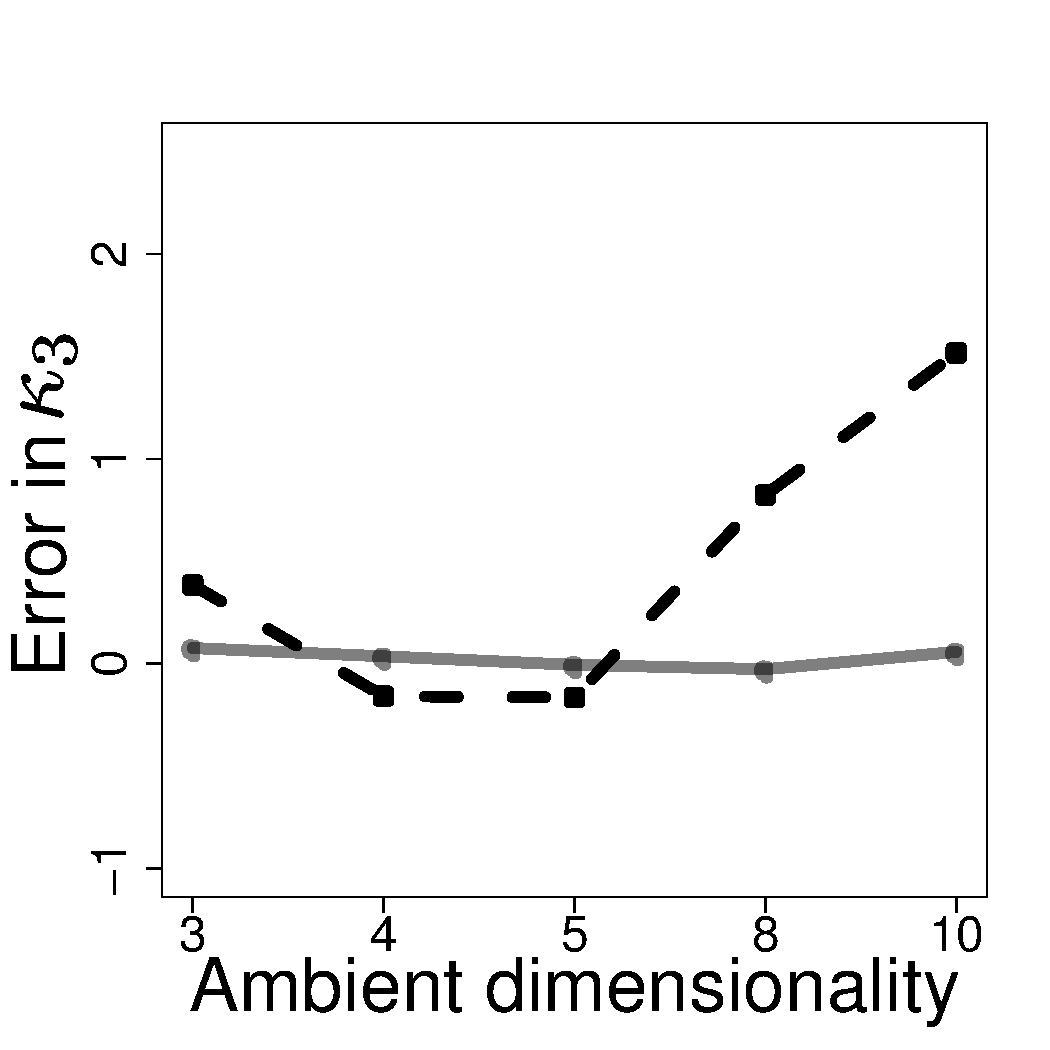
\includegraphics[width=.25\textwidth]{figs/approx_err3_bw.pdf}
\caption{Errors in the posterior mean for the vectorcardiogram
dataset. Each panel is a different component of $\kappa$; solid/dashed lines are the Hamiltonian/approximate sampler.}
  \label{fig:approx_comp}
  \end{figure}

On the vectorcardiogram dataset, the approximate sampler 
is about forty times faster than the exact samplers. For larger
datasets, this difference will be even greater, and the real question is how accurate
the approximation is. Our exact sampler allows us to study this: %we consider different values of $\bkappa$ and 
%different dimensions of the ambient space. In particular, 
we consider the Stiefel manifold $V_{d,3}$,
with the three diagonal elements of $\bkappa$ set to $1, 5 $ and $10$. With this setting of $\bkappa$, and
a random $G$, we generate datasets with $50$ observations, with $d$ taking values $3, 4, 5, 8,$ and $10$.
In each case, we estimate the posterior mean of $\bkappa$ by running the exchange sampler, and treat this as the
truth. We compare this with posterior means returned by our Hamiltonian sampler, as well as the approximate sampler.  Figure \ref{fig:approx_comp}
shows these results. 
%with the three subplots corresponding to the three components of $\bkappa$, and ambient dimensionality
%$d$ increasing along the horizontal axis.
As expected, the two exact samplers agree, and the Hamiltonian sampler has almost no error.
%The approximate sampler is more complicated. 
For values of $d$ around $5$, the estimated posterior mean for the approximate sampler is close to that of the exact samplers. Smaller values lead to an approximate posterior mean that underestimates the actual posterior mean,
while in higher dimensions, the opposite occurs. Recalling that $\bkappa$ controls the concentration of the matrix Langevin distribution about its
mode, this implies that in high dimensions, the approximate sampler underestimates uncertainty in the distribution of future observations.
